\documentclass{beamer}
\usepackage[utf8]{inputenc}
\usepackage[catalan]{babel}

\mode<presentation> {

% The Beamer class comes with a number of default slide themes
% which change the colors and layouts of slides. Below this is a list
% of all the themes, uncomment each in turn to see what they look like.

\usetheme{default}
%\usetheme{AnnArbor}
%\usetheme{Antibes}
%\usetheme{Bergen}
%\usetheme{Berkeley}
%\usetheme{Berlin}
%\usetheme{Boadilla}
%\usetheme{CambridgeUS}
%\usetheme{Copenhagen}
%\usetheme{Darmstadt}
%\usetheme{Dresden}
%\usetheme{Frankfurt}
%\usetheme{Goettingen}
%\usetheme{Hannover}
%\usetheme{Ilmenau}
%\usetheme{JuanLesPins}
%\usetheme{Luebeck}
%\usetheme{Madrid}
%\usetheme{Malmoe}
%\usetheme{Marburg}
%\usetheme{Montpellier}
%\usetheme{PaloAlto}
%\usetheme{Pittsburgh}
%\usetheme{Rochester}
%\usetheme{Singapore}
%\usetheme{Szeged}
%\usetheme{Warsaw}

% As well as themes, the Beamer class has a number of color themes
% for any slide theme. Uncomment each of these in turn to see how it
% changes the colors of your current slide theme.

%\usecolortheme{albatross}
%\usecolortheme{beaver}
%\usecolortheme{beetle}
%\usecolortheme{crane}
%\usecolortheme{dolphin}
%\usecolortheme{dove}
%\usecolortheme{fly}
%\usecolortheme{lily}
%\usecolortheme{orchid}
%\usecolortheme{rose}
%\usecolortheme{seagull}
%\usecolortheme{seahorse}
%\usecolortheme{whale}
%\usecolortheme{wolverine}

%\setbeamertemplate{footline} % To remove the footer line in all slides uncomment this line
%\setbeamertemplate{footline}[page number] % To replace the footer line in all slides with a simple slide count uncomment this line

%\setbeamertemplate{navigation symbols}{} % To remove the navigation symbols from the bottom of all slides uncomment this line
}

\usepackage{graphicx} % Allows including images
\usepackage{booktabs} % Allows the use of \toprule, \midrule and \bottomrule in tables

%----------------------------------------------------------------------------------------
%	TITLE PAGE
%----------------------------------------------------------------------------------------

\title[Short title]{Millora de rendiment d'un sistema d'avaluació de traductors automàtics} % The short title appears at the bottom of every slide, the full title is only on the title page

\author{Ibai Gilabert Rodríguez} % Your name

%\date{\today} % Date, can be changed to a custom date
\date{22 d'abril de 2015}
\begin{document}

\begin{frame}
\titlepage % Print the title page as the first slide
\end{frame}

\begin{frame}
\frametitle{Índex} % Table of contents slide, comment this block out to remove it
\tableofcontents % Throughout your presentation, if you choose to use \section{} and \subsection{} commands, these will automatically be printed on this slide as an overview of your presentation
\end{frame}

%----------------------------------------------------------------------------------------
%	PRESENTATION SLIDES
%----------------------------------------------------------------------------------------

%------------------------------------------------


\section{Introducció}
\begin{frame}
\frametitle{Introducció}
\begin{itemize}
\item Projecte emmarcat en l'àrea del tractament de llenguatge natural (\textit{NLP}). % Concretament, l'avaluació automàtica.

\item El llenguatge natural és inherentment ambigu.

\item Conceptes difosos com ``qualitat'' d'una traducció.
\end{itemize}
\end{frame}


\section{Abast}
\begin{frame}
\frametitle{Abast}
\begin{itemize}
\item Partim d'un sistema funcional: \texttt{ASIYA}

\item Què és pretén aconseguir amb aquest projecte?

\item Quina és la proposta?

\end{itemize}
\end{frame}


\section{Decisions de disseny}
\begin{frame}
\frametitle{Decisions de disseny}
\begin{itemize}
\item El disseny actual no és consistent. %codi acoplat...

\item Aprofitem l'avinentesa: Re-disseny íntegre de TOT el sistema.

\item Paral·lelisme: mètrica i document.

\end{itemize}
\end{frame}


\section{Decisions d'arquitectura}
\begin{frame}
\frametitle{Decisions d'arquitectura}
\begin{itemize}
\item Opció \textit{GPU}.

\item Opció \textit{Cluster} de computació

\end{itemize}
\end{frame}


\section{Resultats}
\begin{frame}
\frametitle{Resultats}
%Uncomment the code on this slide to include your own image from the same directory as the template .TeX file.
\begin{figure}
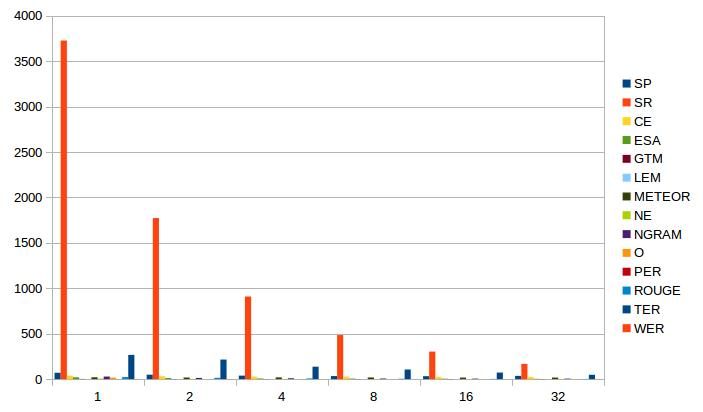
\includegraphics[width=\linewidth]{resources/chart_presentation.jpg}
\end{figure}
\end{frame}


%------------------------------------------------

\begin{frame}
\huge{\centerline{Preguntes}}
\end{frame}

%----------------------------------------------------------------------------------------

\end{document} 